\documentclass[a4paper,11pt]{article}
\usepackage[francais]{babel}
%% Prévu pour compiler avec lualatex
% \usepackage[utf8]{inputenc}
\usepackage{fontspec}
%\usepackage{libertine}
% \usepackage[T1]{fontenc}
\usepackage{graphicx}
\usepackage{fancyhdr}
\usepackage[top=2.5cm, bottom=2.5cm, left=2cm, right=2cm]{geometry}
\usepackage{listings}
\usepackage[utf8]{luainputenc}
\usepackage[hidelinks]{hyperref}
\usepackage{caption}

\lfoot{\bsc{Enseirb-Matmeca}}
\rfoot{Informatique --- 3\ieme{} année}

\pagestyle{fancy}
\begin{document}

\begin{titlepage}
  \begin{center}

    \begin{center}
      
\includegraphics[width=4cm]{EM.jpg}
    \end{center}

    \vspace*{1cm}
        
    \rule{0.75\linewidth}{0.7mm}\\[0.4cm]
    {\Huge Rapport TP2 --- MPI\\[0.4cm]}
    \rule{0.75\linewidth}{0.7mm} \\[1.5cm]

    {\Large Bazire \bsc{Houssin}\\Sylvain \bsc{Vaglica}\\Stéphane \bsc{Castelli}\\[2cm]}
    {\Large Mardi 5 Novembre 2013}
  \end{center}
\end{titlepage}

\tableofcontents
\clearpage
\section{Introduction}



\section{Présentation de l'algorithme}
L'algorithme de calcul séquetiel pour calcul de forces gravitationnelle sur un système de $n$ masses distinctes, consiste à répéter pour chaque masse $m$ les étapes suivantes:\\

\begin{itemize}
\item Pour chaque masse $m'$ distincte de $m$, calculer la force d'intéraction gravitationnelle entre les deux masses.
\item Calculer la force résultante (direction et norme) de toutes les autres masses sur $m$.
\item Trouver la distance minimale entre n'importe quelle paire des masses.
\item Calculer l'accélération résultante de la masse $m$.
\item En déduire sa vitesse, le pas de calcul ($dt$) et sa nouvelle position.
\end{itemize}
\\
Les formules utilisées pour l'accelération, la vitesse et de la position sont celles obtenues par l'application du principe fondamental de la dynamique sur chacune des masses.

Pour la version distribuée, le stockage de l'ensemble des masses est réparti en nombre égal sur l'ensemble des processus. Chaque processus effectue les calculs sur les masses qu'il possède en local, mais doit régulièrement envoyer les données aux autres processus. La topologie et les communications seront décrites dans la partie suivante. On obtient donc l'algorithme suivant, à appliquer sur chaque masse $m$ locale:\\
\begin{itemize}
\item On déterminer tout d'abord le pas de calcul (commun à tout les processus), grâce à la distance minimale entre tous les couples de masses mémorisée à l'itération précédente.
\item Pour chaque masse  reçue $m'$ distincte de $m$, calculer la force d'intéraction gravitationnelle entre les deux masses.
\item Calculer l'accélération de la masse $m$, induite par $m'$.
\item En déduire sa vitesse et sa nouvelle position induite par $m'$.
\end{itemize}

Pour chacun des deux algorithmes, on peut itérer indéfiniement afin d'obtenir une trajectoire de chacune des masses plus ou moins longues. Dans les deux cas, on effectue un premier tour de boucle sans modifier les positions afin de déterminer le pas de calcul qui est donné par la formule: (STEPHANE: METTRE LA FORMULE DU dt ICI).

\section{Topologie, répartition des données et communications}
 
\section{Performances}

\begin{figure}[h!]
  \centering
  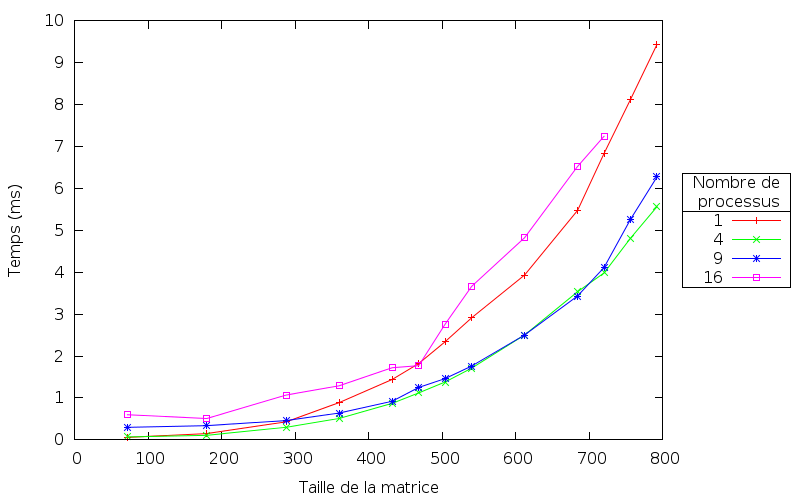
\includegraphics[width=\textwidth]{plot.png}
  \caption{Performance du programme}
  \label{perf}
\end{figure}


\section{Conclusion}


\end{document}
